\documentclass[12pt]{article}
%\usepackage{kpfonts}
\usepackage{graphicx}
\usepackage{float}
\usepackage{algorithm}
\usepackage{amsmath}
\usepackage[noend]{algpseudocode}
\usepackage{amssymb}
\usepackage{bm}

\makeatletter
\def\BState{\State\hskip-\ALG@thistlm}
\makeatother

%\algnewcommand\algorithmicforeach{\textbf{for each:}}
%\algnewcommand\ForEach{\item[ \algorithmicforeach]}

\algnewcommand\algorithmicforeach{\textbf{for each}}
\algdef{S}[FOR]{ForEach}[1]{\algorithmicforeach\ #1\ \algorithmicdo}

\DeclareMathOperator*{\argmin}{\arg\!\min}
\DeclareMathOperator*{\argmax}{\arg\!\max}

\begin{document}

\begin{center}

Document Classification Pipeline


\end{center}

\section{Introduction}
In an effort to fascilitate multidisciplinary research within the University of Texas at El Paso, we have developed a methodology
to automatically assign or recommend communities of practice to faculty. A community of practice is a group comprised of several
faculty members in which they direct their research towards a same research topic. These topics may range from Cyber Security to Smart Cities.
In order to make these community assignments or recommendations as meaningful and satisfactory to the faculty member as possible, recommendations
are to be based on the contents of the faculty's research publications knowledge of research topic interests.

In this text, we propose a document summarization method based on semantic relations in the text. We analyse the effectiveness of
this compressed document representation as input to a learning algorithm such as a neural network in a text classification task.
We then provide an analysis on the performance of modern convolutional neural networks on multiple publication datasets, and provide discussion
on the effectiveness of network architecture and choice of hyperparamters. Afterwards we analyse performance of a learning model motivated by
the initial document summarization work discussed earlier in the text.
Finally, we integrate all work into a classification system to assign faculty members to communities of practice based on their publication data.


\subsection{Problem Definition}
Academic publications are often the product of interdisciplinary research. Consider the scenario where a co-author collaborates
in a publication due to technical expertise in a field other than the focus of the publication e.g. computer vision applied in a biology publication.
Additionally, communities of practice are usually groupings of faculty members from mixed areas of research interest and expertise.
In order to make meaningful membership suggestions based on a co-author's publications, it is of great value to identify the relevant text when
using these data to assign him or her into a community of practice.
This is because we want to suggest membership to communities of practice based on meaningful information, considering only the text
which is relevant to this specific co-author. Traditional vector space models represent a document as a vector of identifiers or statistics,
but lose context and may not accurately represent a publication with respect to the interest of the specific co-author.
This motivates us to explore embedding based features for classification tasks, alongside convolutional neural networks.
Convolutional neural networks are known for their ability to learn high-level features from their input data.
We explore the effectiveness of embedding-based representations of data using neural network models on classification tasks.

First, we propose a simple algorithm for extracting a set of words from text. These words are selected based on minimizing a criteria inspired by semantic
relations in sentence neighborhoods. We then provide some analysis and justification for our method, and later return to a neural network adaptation to
this keyword extraction algorithm.

\section{Related Work}
Our proposed feature extraction method relies on extracting words which are considered keywords. We do this considering semantic similarity rather
than term frequency information.
Common keyword extraction techniques include:
\begin{itemize}
  \item TF-IDF
  \begin{itemize}
    \item Weighs a term positively based on frequency, weighs a term negatively based on number of documents the term occurs
    \item Ignores any type of relationships with other terms in the document
    \item Relies on frequency within the document, and within the corpora
    \item Assumes a keyword will frequently appear on a document, but not within other documents in the corpus
  \end{itemize}
  \item Word Co-Occurrance Relationships
  \begin{itemize}
    \item Model the relevance of each word from each document as s Markov Chain with states \textit{C} and \textit{T}
    \item Transition from \textit{C} to \textit{T} is the number of times the term occurs in a document \textit{d} divided by the number of times the term occurs in all documents
    \item Transition from \textit{T} to \textit{C} is the number of times the term occurs in a document \textit{d} divided by the number of term occurrences in \textit{d}
    \item If two terms share similar transition probabilities, they are considered related
    \item A term is considered a keyword if its transition probabilites are diverging from the so called \textit{background} distribution, or the set
    of the most common transition probabilites
  \end{itemize}
  \item Latent Dirichlet Allocation
  \begin{itemize}
    \item Topic modeling technique
  \end{itemize}
  \item Non-Negative Matrix Factorization
\end{itemize}

Vector space models are those that represent text as a vector of statistics or identifiers. Vector space models include:
\begin{itemize}
  \item One-hot representation of words
  \item Term Count vectors
  \item TF-IDF vectors
\end{itemize}
The vector space models, although effective, have limitations such as:
\begin{itemize}
  \item Long documents are poorly represented because they have poor similarity values (a small scalar product and a large dimensionality)
  \item Documents with similar context but different term vocabulary won't be associated
  \item Term order in the document is lost in the vector space representation. No context preservation
  \item Assumes terms are independent. Does not exploit context any kind. Weighting is intuitive but not formal
\end{itemize}


\section{Keyword Extraction Methodology}

In order to convert a word into a dense, real-valued vector, we use a token-to-embedding dictionary to map a token to its corresponding embedding form.
This dictionary is typically obtained after learning a language model using a neural network. One property of this word embedding space is that
words can now be represented as points in Hilbert space. Another property and perhaps the most important is that semantic relationships are captured,
in this embedding space and can be measured between any two words using the cosine similarity metric. This is an attractive property that
allows for term comparison by semantic relationships. These relationships can range from complete similarity i.e. the same term, to term orthogonality
i.e. unrelated words, and even capture the direction of the relation e.g. negative values of cosine similarity.

The cosine similarity between two vectors can be computed as follows:

\[
  \frac{\mathbf{x} \cdot \mathbf{y}}{\lVert \mathbf{x} \rVert \lVert \mathbf{y} \rVert}
\]

If we normalize all embeddings to have unit norm, then the cosine similarity between two words is simply a dot product computation.

\subsection{Keyword Extraction}
We propose a word embedding based feature vector representation of text document. We wish to measure performance of classifiers when trained using sequences of these
extracted keywords. Our intuition is that we can compress a document's main ideas using a small set of keyword embeddings. This set of keywords can in turn
be determined entirely from semantic relations within the text. In other words, we aim to extract these keywords ignoring frequency or hand-engineered
indications, but rather looking for strong semantic similarities within candidate keywords.

As described in previous sections, popular feature extraction methods for text classification involve count or frequency based feature representations with respect to
a predetermined vocabulary. This method, although effective, fails to capture semantic relations and concepts within the text.

This feature representation of text is highly interpretable. A simple dictionary lookup can map word embeddings into words.
The main purpose of our framework is to provide community membership recommendations to faculty members
based on their publications. Having the faculty member read and interpret the features used for membership prediction is of great value,
as the faculty is able to interpret a classifier's decision as a function of the input data.

We restrict our search for keywords to look only in noun phrases. In other words, when analysing a sentence, we only consider text which is
part of a noun phrase, and ignoring all other text in the sentence. The reasoning behind this design decision is:
\begin{itemize}
\item A filtering mechanism is essential for reduced running time. Avoiding processing of the entire sentence text, ignoring non-informative text
helps in greatly reducing computation time.
\item A noun phrase is likely to contain keyword tokens. These can be found in multiple forms e.g. adjectives or nouns. By ignoring tokens which
are not likely to be keywords or part of a keyword phrase e.g. \"cloud computing\" or \"deep learnign\", we reduce the amount of noise in our keyword
selection scheme.
\end{itemize}

Of course, this assumption comes with the risk of discarding or ignoring possible keyword tokens. This is true because chunker misclassification
may cause our system to ommit a candidate keyword tokens because it was not labeled to be part of a noun phrase.

Given a document, our keyword extraction algorithm works as follows:
\begin{itemize}
\item Remove non-alphanumeric characters and convert to lowercase.
\item Tokenize each sentence into a list of words.
\item Perform Part of Speech tagging on each list of words i.e. sentence
\item Chunk each sentence into noun phrases.
\item Map each token in each noun phrase to its corresponding word embedding vector.
\item Perform Mean Cosine Similarity Minimization to extract a keyword noun phrase for each sentence.
\end{itemize}


\subsection{Algorithms}
\begin{algorithm}[H]
\caption{Extract Keyword Noun Phrase from a Sentence}
\begin{algorithmic}[1]
\Procedure{MeanCosineSimilarityMinimization}{$\{\{np^{1}_{1}, ...,np^{1}_{|np^{1}|}\}, ..., \{np^{n}_{1}, ...,np^{n}_{|np^{n}|}\}\}$}
\For {$k$ = 1 to $n$}
\State$ \bm{C^k} = \begin{bmatrix}
         np^{k}_{1} \\
         \vdots \\
         np^{k}_{|np_k|} \\
        \end{bmatrix} \times  \begin{bmatrix}
         np^{k}_{1} \\
         \vdots \\
         np^{k}_{|np_k|} \\
        \end{bmatrix}^{T}$

\State$c_{k} = \frac{1}{|np_i|^2} \sum^{|np_i|}_{i=1} \sum^{|np_i|}_{j=1} \bm{C^{k}_{(i,j)}}$
\EndFor

\Return $\argmin\limits_{k} c$
\EndProcedure
\end{algorithmic}
\end{algorithm}

The procedure \textit{MeanCosineSimilarityMinimization} receives as input a set of noun phrases
$ \mathbf{np^i} = \{np^i_1, ..., np^i_{ | \mathbf{np^i}|} \}$ corresponding to the \textit{i}th sentence. Each noun phrase $np^i_1$
is comprised of one or more word embedding vectors, corresponding to the noun phrase's tokens mapped to their vector representations.
For each noun phrase $np^i_1$, we compute the average cosine similarity between all the noun phrase's tokens. The algorithm returns the noun phrase which
minimizes its average cosine similarity metric. The reasoning behind this noun phrase selection algorithm is as follows. A noun phrase with a very informative
token i.e. word embedding will contain a token which will stand out from the rest of the tokens in the noun phrase. We assume that this can be measured
by low cosine similarity between an informative token and all its other noun phrase tokens. We therefore compute, for all noun phrases in a sentence,
the mean \textit{within-noun-phrase} average cosine similarity, as described in algorithm 1.



\subsection{Dataset Description}
We use the "NSF Research Award Abstracts 1990-2003" dataset found in UCI's machine learnine dataset repository.
This dataset contains 129,000 research abstract texts, along with corresponding metadata. For our research purposes, we only
consider the abstract text and the corresponding class label. We remove non-alphanumeric characters and words which are not in a
specified set of part of speech tags.\\

We use the Stanford NLP department's GloVe embedding dataset for transforming words into vectors.


\section{Performance Analysis}
In the following sections, we provide performance analysis and discuss strengths and shortcomings of our method. We begin by analysing keyword extraction,
and follow with classification performance.
\subsection{Keyword Extraction}
We verify the relevance of keywords obtained through our and other keyword extraction methods by measuring their average recall, precision, and fmeasure
from a set of abstracts with author-provided keywords. In order to make the distinction from keyword noun phrases extracted through our method and paper keywords
provided by the authors, we refer to these author provided keywords as \textit{paper keywords}. We stem all extracted and paper keywords for evaluation purposes.

\begin{itemize}
\item For each \textit{paper keyword}:
\begin{itemize}
  \item Search for the \textit{extracted} keyword noun phrase with the highest number of equal tokens as the paper keyword.
  Denote this keyword noun phrase as \textit{selected keyword}. Denote the number of same tokens in \textit{selected keyword} as the
  paper keyword as the number of \textit{hits}.
  \item precision = hits/number of tokens in \textit{selected keyword}
  \item recall = hits/number of tokens in \textit{selected keyword}
  \item fmeasure = 2*((precision*recall)/(precision+recall)). If both precision and recall are 0, f-measure = 0.
\end{itemize}
\item Compute average precision, recall, and f-measure
\end{itemize}

Selected keywords with a large number of tokens e.g. five are more likely to have higher recall, or have a higher chance of having keyword \textit{hits}.
This however is countered-balanced by being more likely to have smaller precision i.e. large number of tokens that don't \textit{hit}
paper keyword tokens. In the end, we consider f-measure as an indication of performance. Two important points are worth mentioning:
\begin{itemize}
\item Extracted keywords which are not \textit{paper keywords} are not necessarily uninformative, non-relevant, or noise.
\item Many \textit{paper keywords} are not explicitly found in their corresponding abstract's text. This means that there are bound to be multiple
paper keywords that will not receive any hits, since the keyword extraction methods used make no predictions and only extract tokens found in the text.
\end{itemize}

The first point provides a sort of justification for extracted tokens which are not \textit{paper keywords}.
The performance values computed are not indicative of a particular keyword extraction method being better or worse than others. We compute these
performance values in order to validate and verify that our keyword extraction method manages to capture and extract what the authors considered to
be relevant and \textbf{key} words. The second point gives insight to the extent of the computed performance values' meaning. Of course, we consider high performance
values in this particular case to be positive. This is indicative of keywords the authors considered to be important being successfully extracted. There are
however many cases in which the paper keywords are not present, so that in itself diminishes the importance of the computed performance values.
Overall, we consider the \textbf{average} performance metric values, and this second point affects all keyword extraction methods used equally.

\begin{figure}[H]
\centering
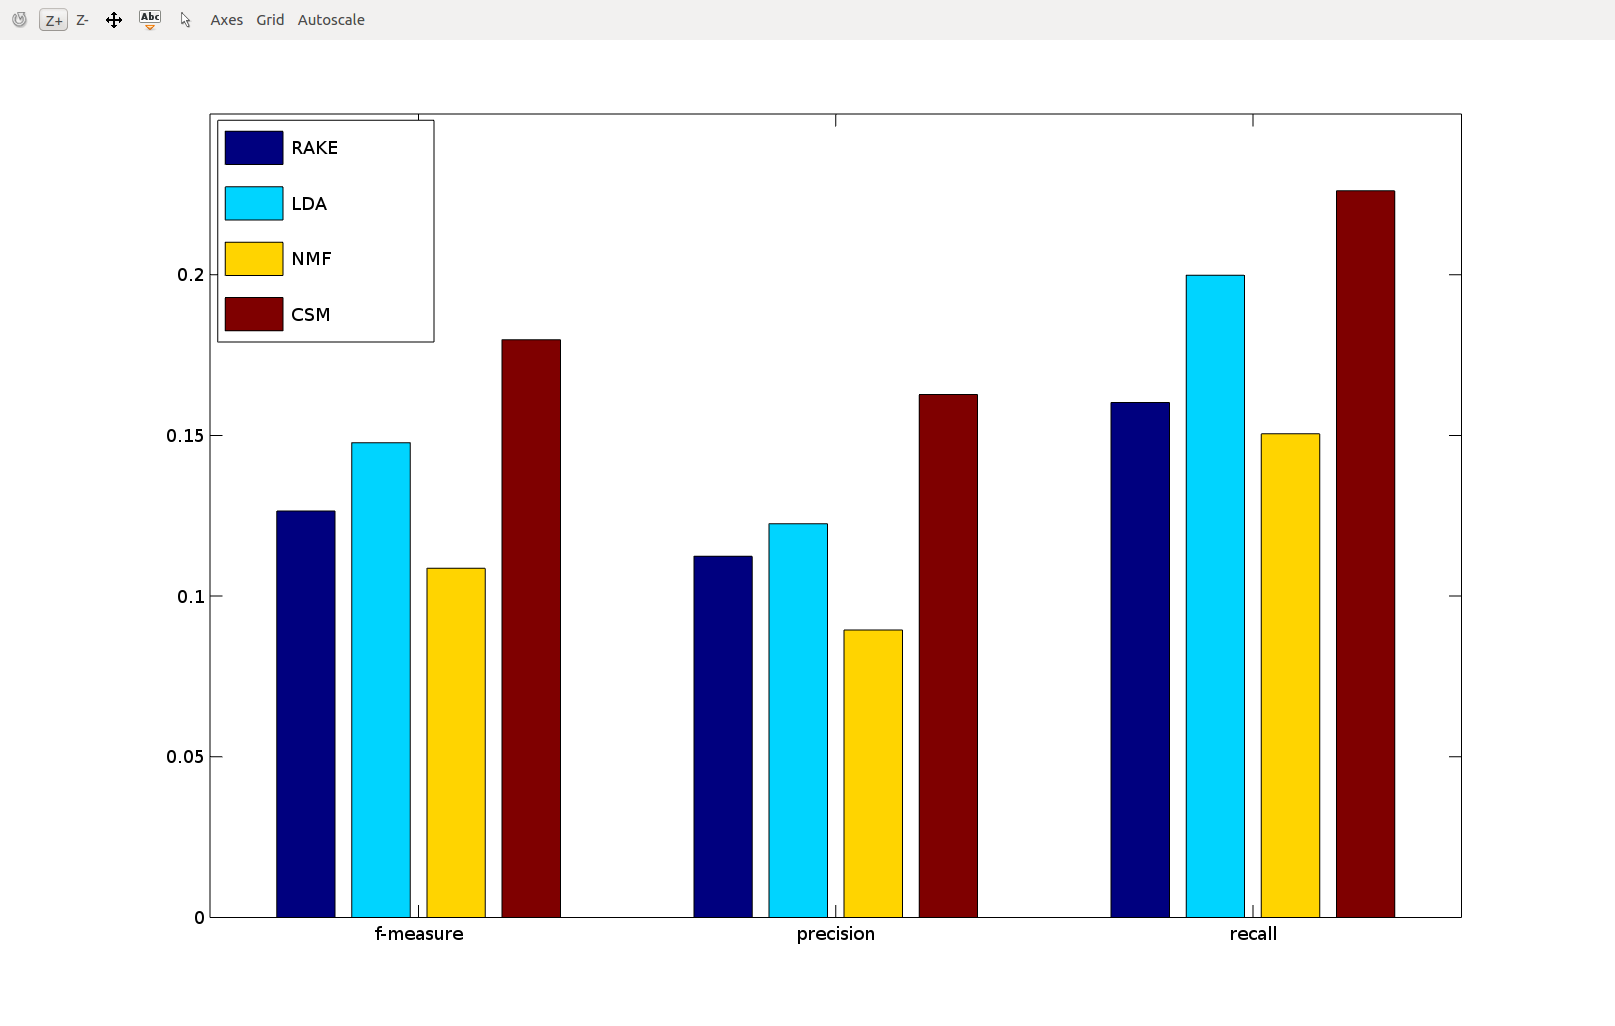
\includegraphics[height=2in, width=4in]{Images/keywordresults.png}
\caption{Bar plot of f-measure, precision, and recall values computed for RAKE, LDA, NMF, and Cosine Similarity Minimization respectively.}
\end{figure}


\subsection{Classification Performance}

We now present classification performance using our proposed feature representation, and compare against classifier performance using
frequency based features.
\begin{tabular}[pos]{l c}
  \textbf{Baseline: TF+SVM} & \textbf{0.876}\\
  5-NN & 0.779\\
  Random Forest & 0.779\\
  MLP (Logistic) & 0.750\\
  MLP (ReLU) & 0.721\\
  MLP (ReLU) 100,100 & 0.780\\
  MLP (ReLU) 200,150, 100, 50 & 0.783\\
  MLP (ReLU) 400,300,200,100,50,10 & 0.815\\
\end{tabular}

The multilayer perceptron achieves the highest performance of all models trained using our embedding based features. This neural
network had hidden layer sizes of 400, 300, 200, 100, 50, and 10 respectively. We used Rectifier Linear Units (ReLU) for non-linearities.
As mentioned previously, our classification scheme is to classify each individual trigram
\begin{figure}[H]
\centering
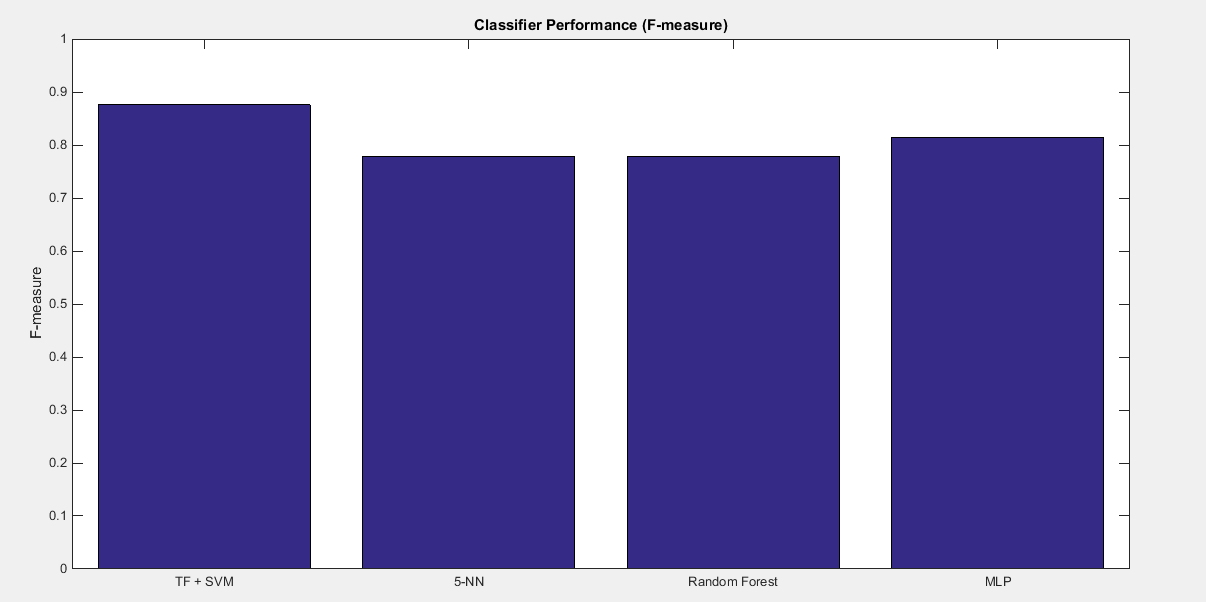
\includegraphics[height=2in, width=4in]{Images/classifier_fmeasure.png}
\caption{Bar plot of f-measure values obtained with frequency based features and a SVM, as well as models trained with our proposed embedding based features.
The multilayer perceptron achieved the highest performance out of all the models trained with our proposed features.}
\end{figure}


\section{Communities of Practice: Learning to Classify Publication Data}
Our next efforts focus on learning to classify faculty publication data. We explore text classification
using convolutional neural networks and word embeddings, and compare performance with popular text classification methods
such as TFIDF with Linear SVM.

\subsection{Convolutional Neural Network for Text Classification}
In order to exploit context and semantic relations in the text, we use embeddings for classification.
We train a convolutional neural network using word embeddings and applies convolutions on sliding
receptive fields for context exploitation. In order to feed our neural network with text data, we transform it to a vectorial
representation, a sequence of word indexes.

For each abstract in our dataset, we map its words to a sequence of word indexes,
so that each word is replaced by an integer identifier. This mapping is contructed with a tokenizer based on occurance statistics.
It should be noted that the only use for this tokenizer is to create integer identifiers for words. The value of the integer
itself means nothing more than a word index. We then zero-pad or truncate our integer sequences to have a specified sequence length. This is
a common practice when processing data as inputs to a neural network to provide a sort of input protocol or standard to the net.

\begin{figure}[H]
\centering
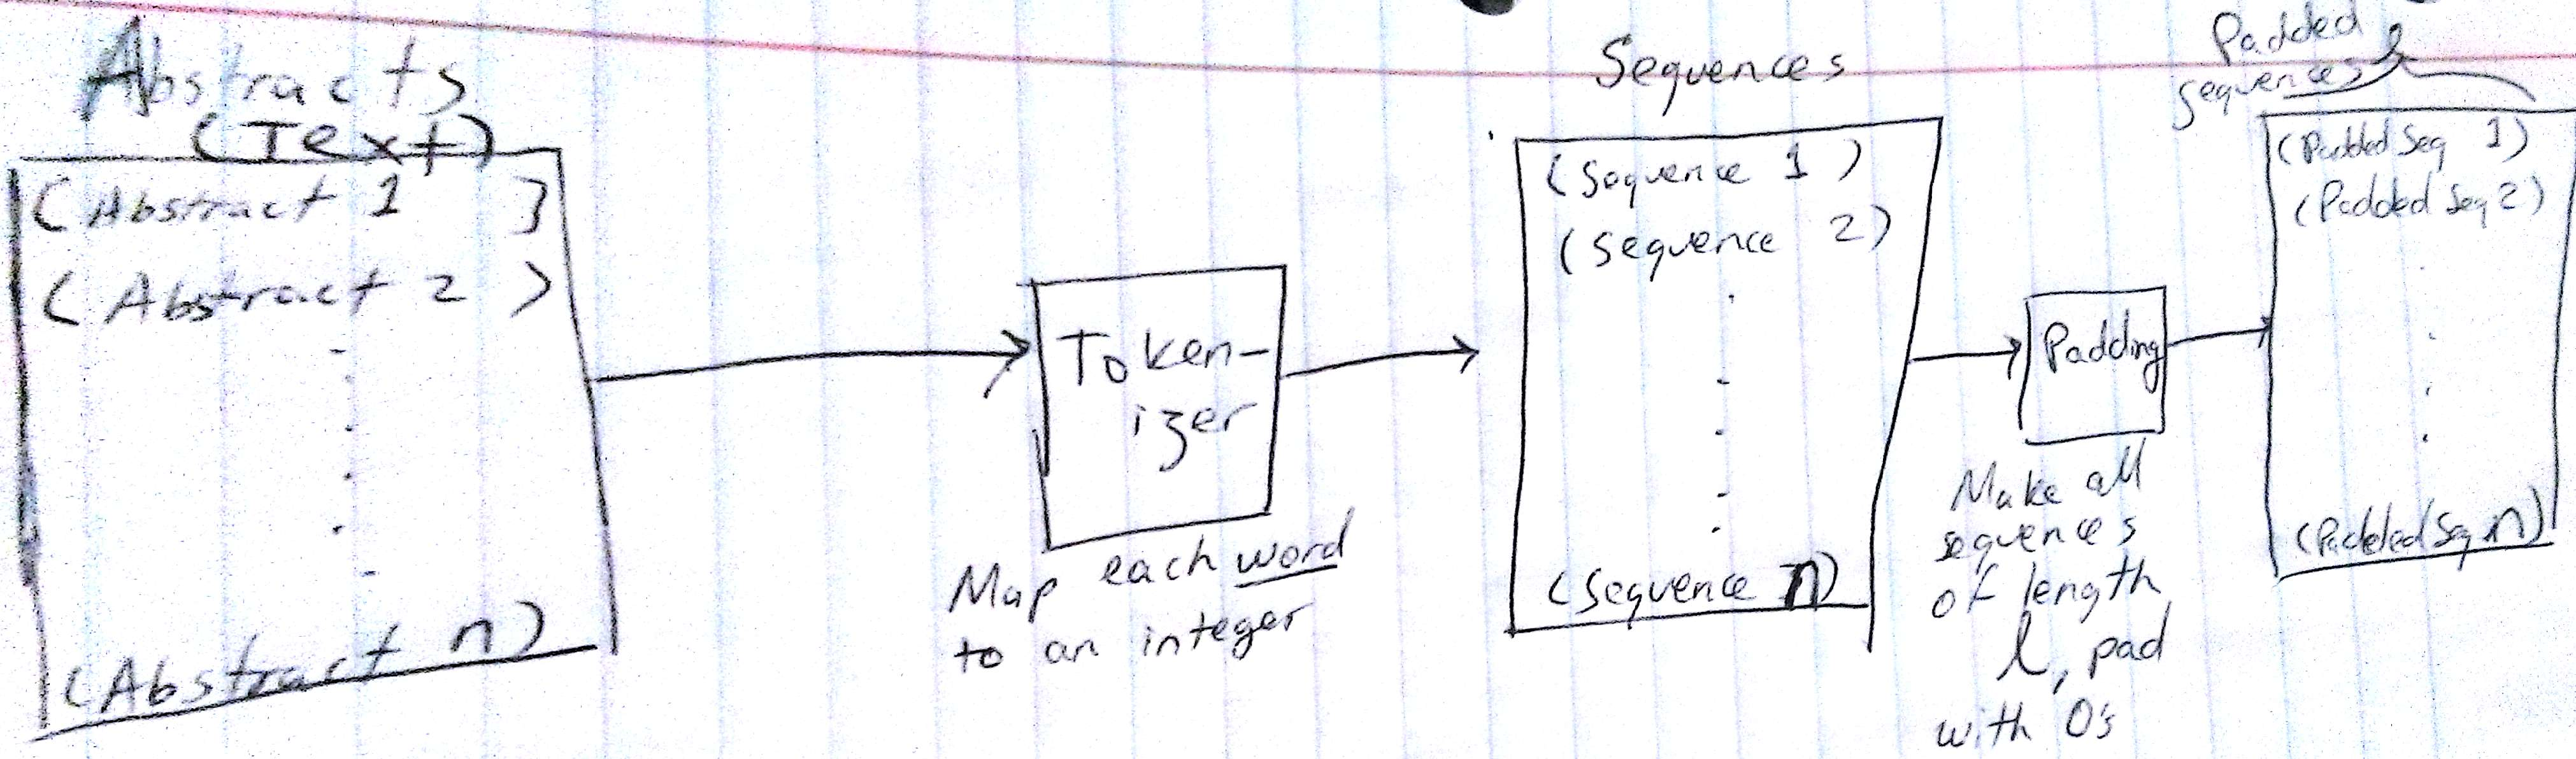
\includegraphics[height=2in, width=4in]{Images/abstracts_to_sequences.jpg}
\caption{Abstract text is mapped to a padded sequence of word indexes.}
\end{figure}




We use an embedding layer as the input layer to our convolutional network. This layer maps a sequence of word indexes i.e. integers
to a sequence of embeddings i.e. vectors.
Concretely, the network's input layer, the embedding layer, receives as input a sequence of integers and outputs a sequence of word embeddings.
We initialize the embedding layer using the pretrained embeddings from the GloVe dataset. We also restrict the size of our embedding
layer to have at most a specified amount of words, determined when we build our sequence dataset. We also perform finetuning on these
initial embedding values, meaning they are modified as normal parameters in a neural net would during training.

\begin{figure}[H]
\centering
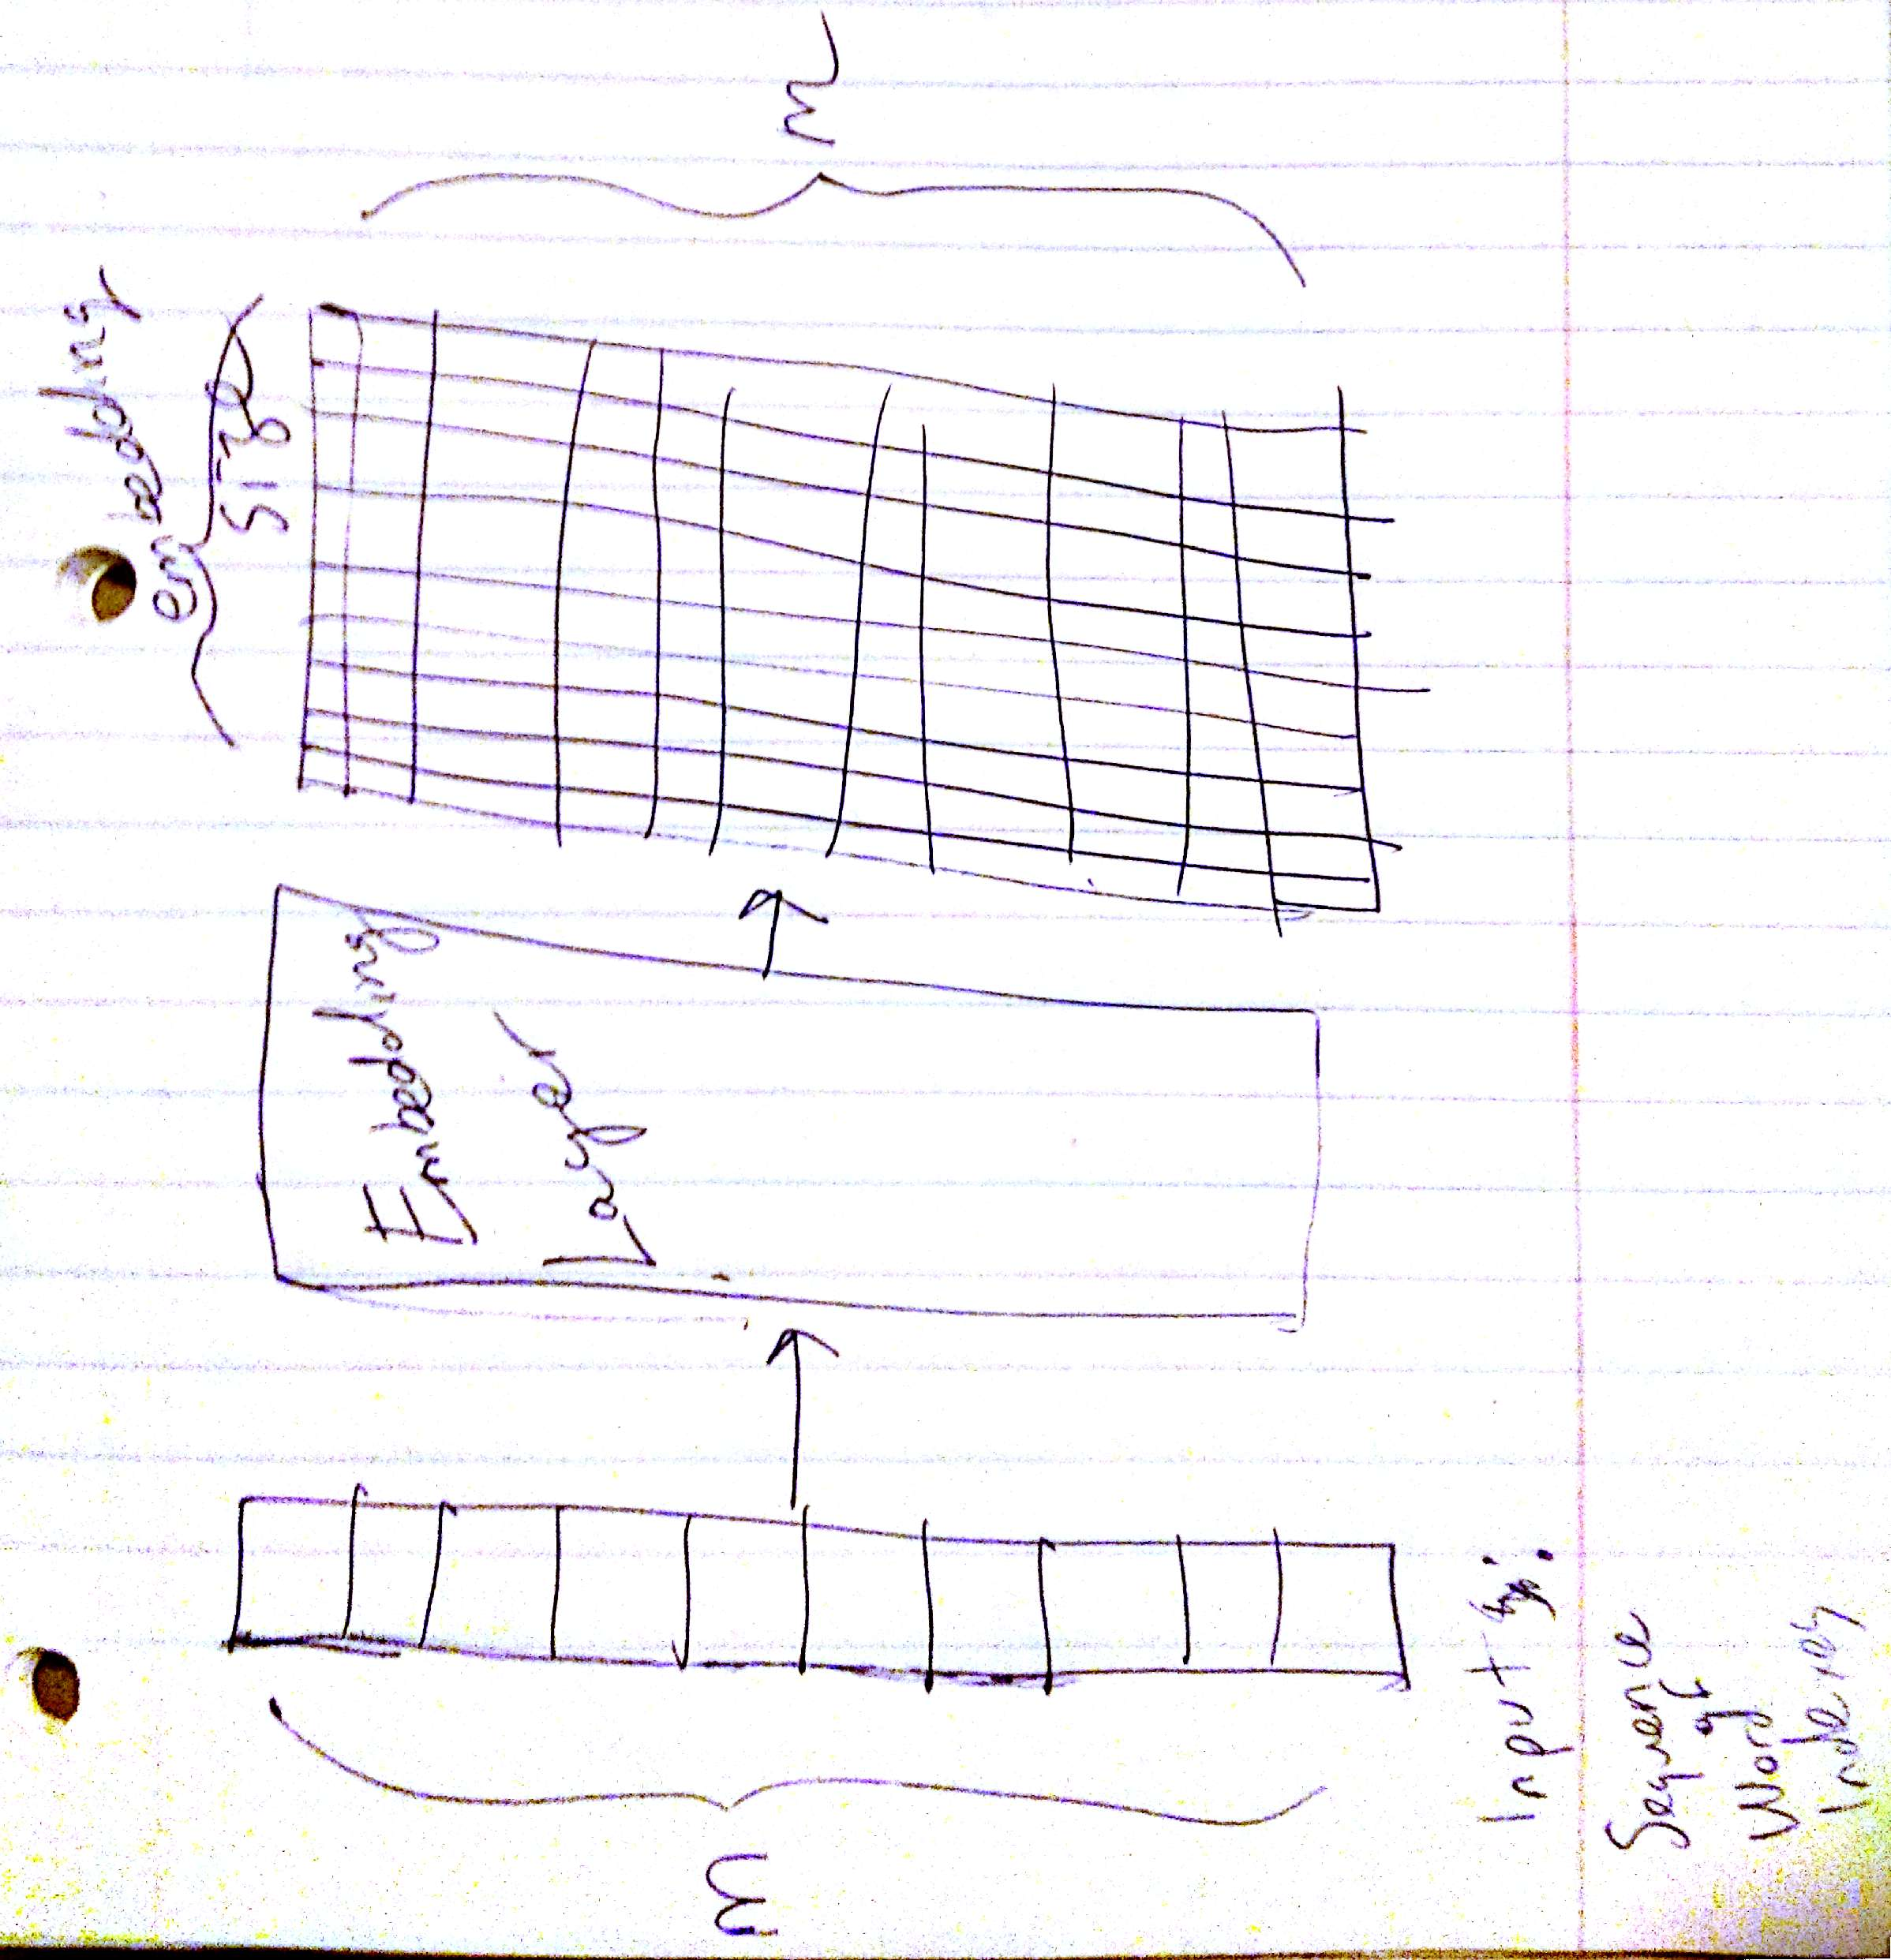
\includegraphics[angle=270,origin=c,height=2in, width=4in]{Images/sequences_to_embeddings.jpg}
\caption{Example of a network's input. The network receives as input a sequence of word indexes i.e. integers maps that sequence to a sequence of word embeddings, one per
word index.}
\end{figure}

Our neural network's pipeline follows conventional convolution and pooling operations. We convolve filters on sliding regions or 'receptive fields'
of the transformed data to capture context and extract high level features.

\begin{figure}[H]
\centering
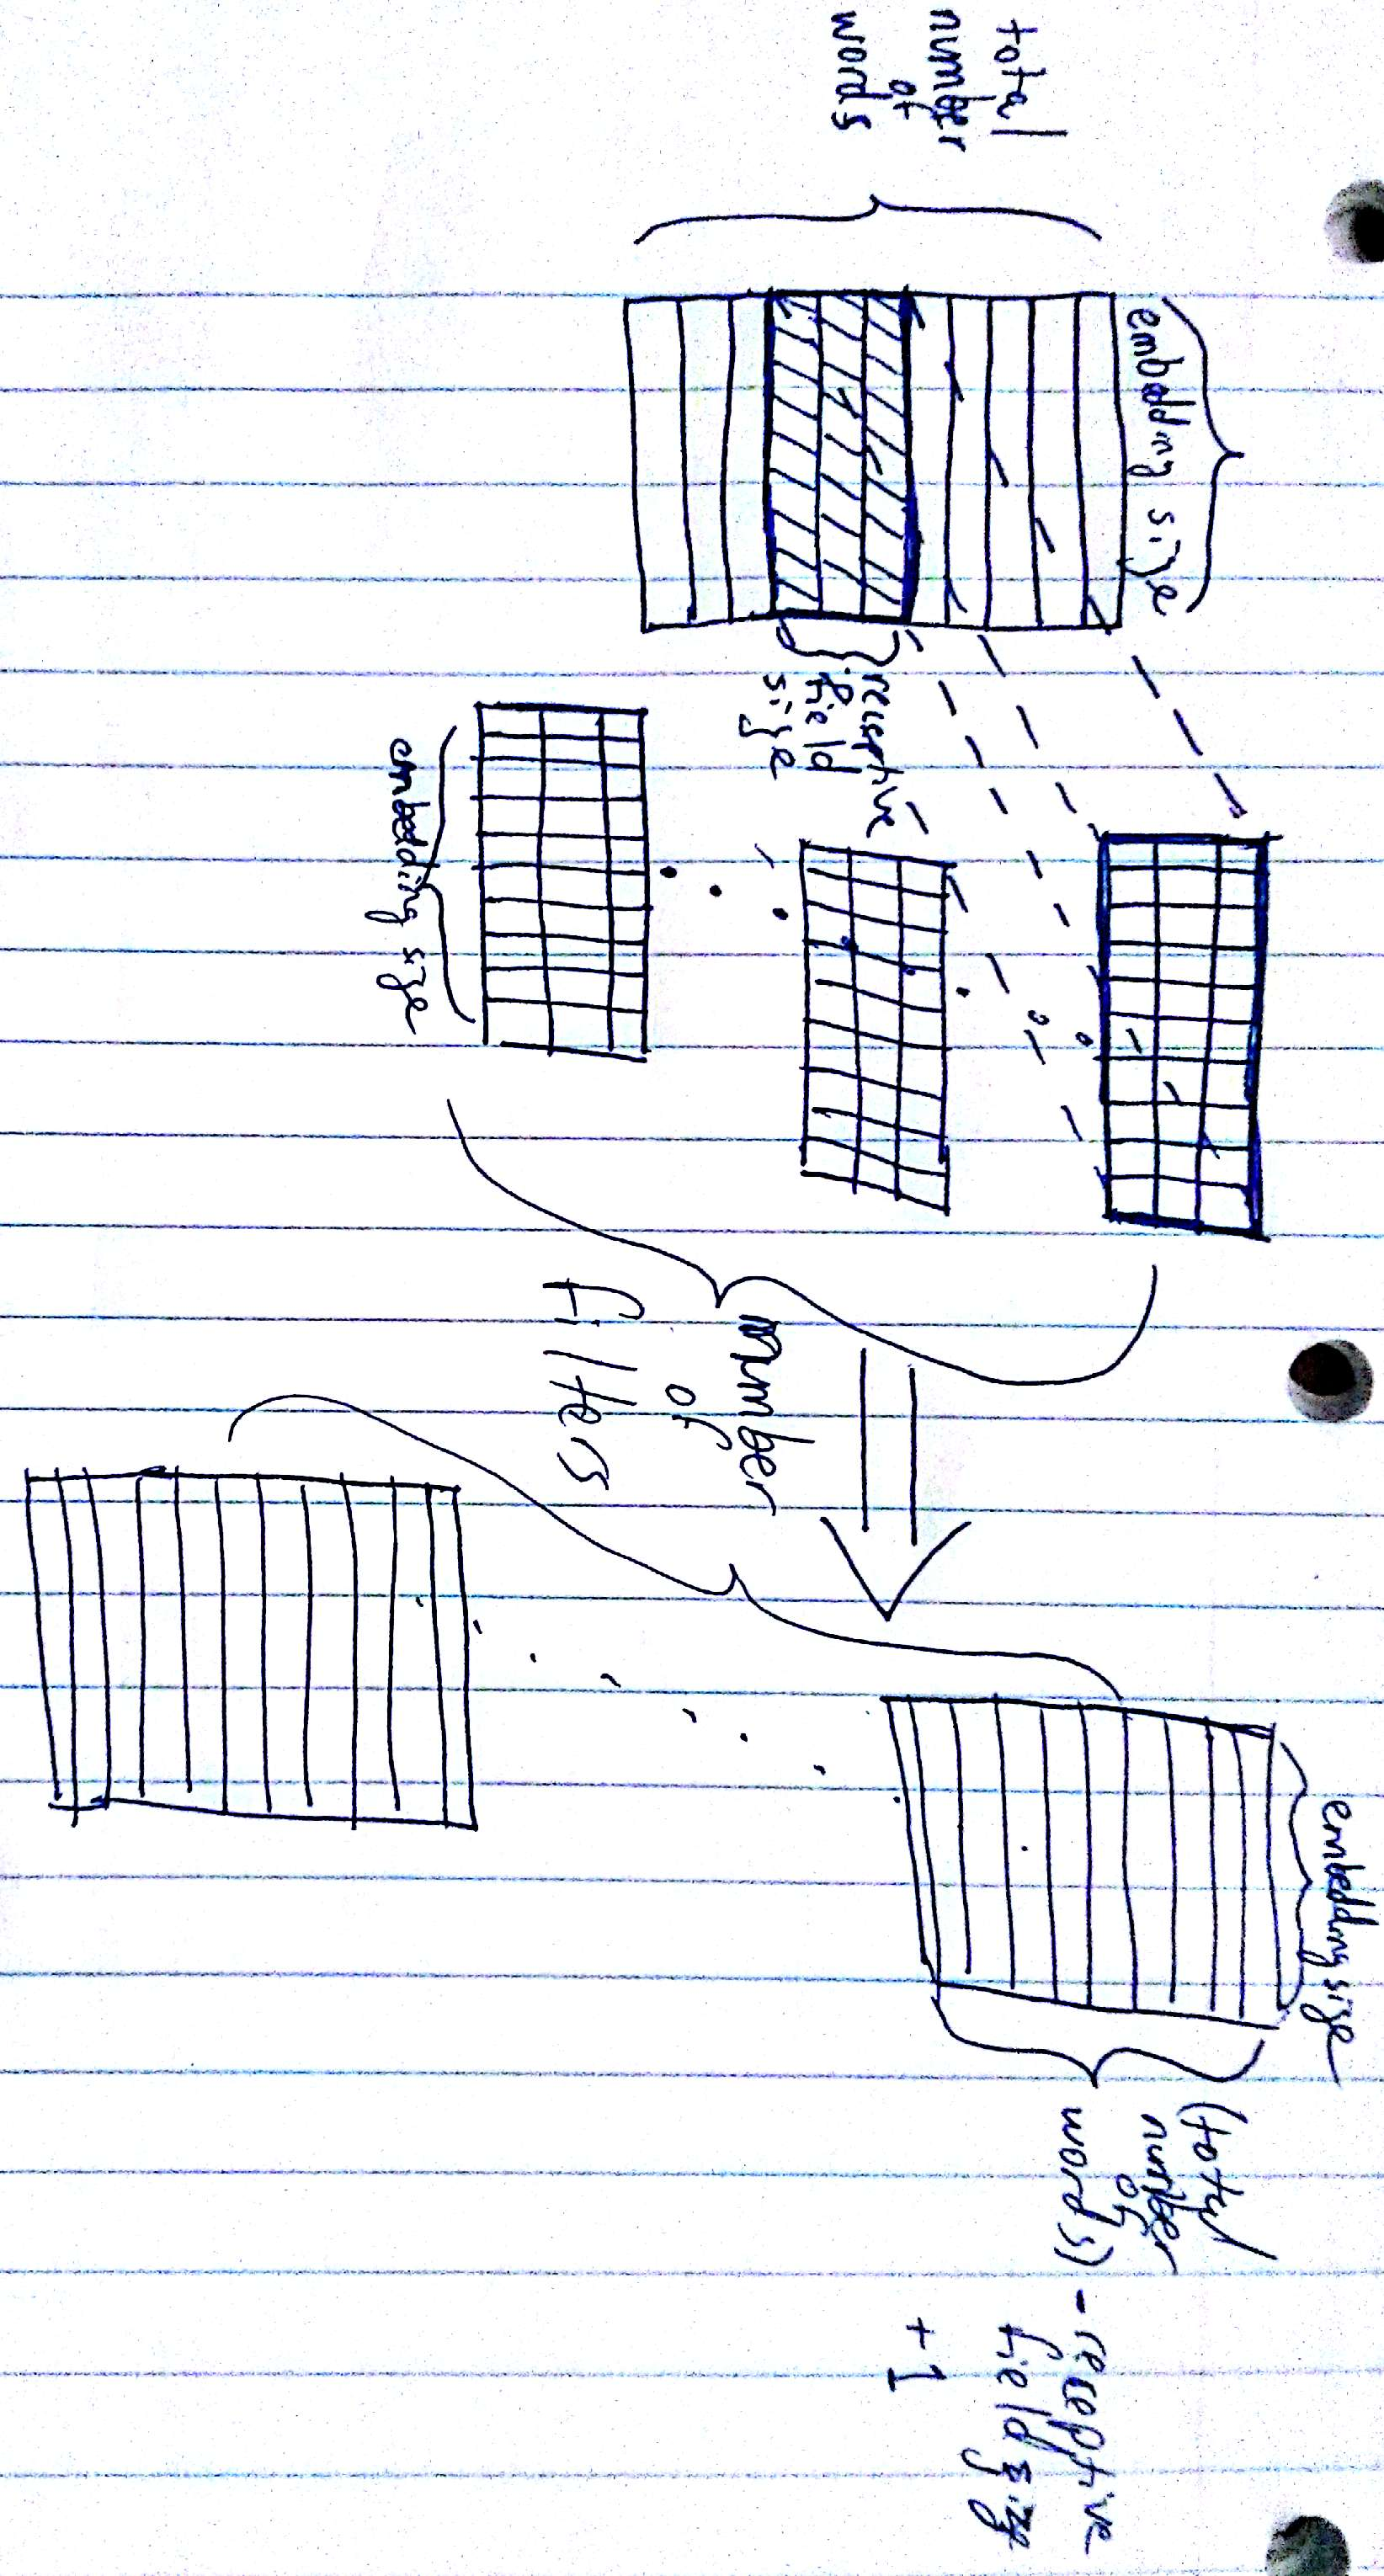
\includegraphics[angle=90,origin=c,height=2in, width=4in]{Images/convolution_figure.jpg}
\caption{After applying the embedding mapping operation, we convolve the data with filter to create 'feature maps'. We use sliding receptive fields to
capture context within the text.}
\end{figure}

\subsection{Convolutional Neural Network for Text Classification}
We train a convolutional neural network for classifying our text data. The first hidden layer is an Embedding layer,
which maps an input sequence of word indexes to a matrix of word embeddings, stacked row-wise. The embedding layer is initialized
using the GloVe embeddings, but the values are further fine-tuned as part of the neural network's parameters.
Following the Embedding layer, we use conventional feature maps, comprised of convolution-pooling layer pairs.
Each feature map is a convolutional/pooling layer pair.
We add a Long Short Term Memory layer as the last hidden layer, followed by a softmax output layer.
This layer is adequate for sequence data, as is the case in sequences of text.

\begin{figure}[H]
\centering
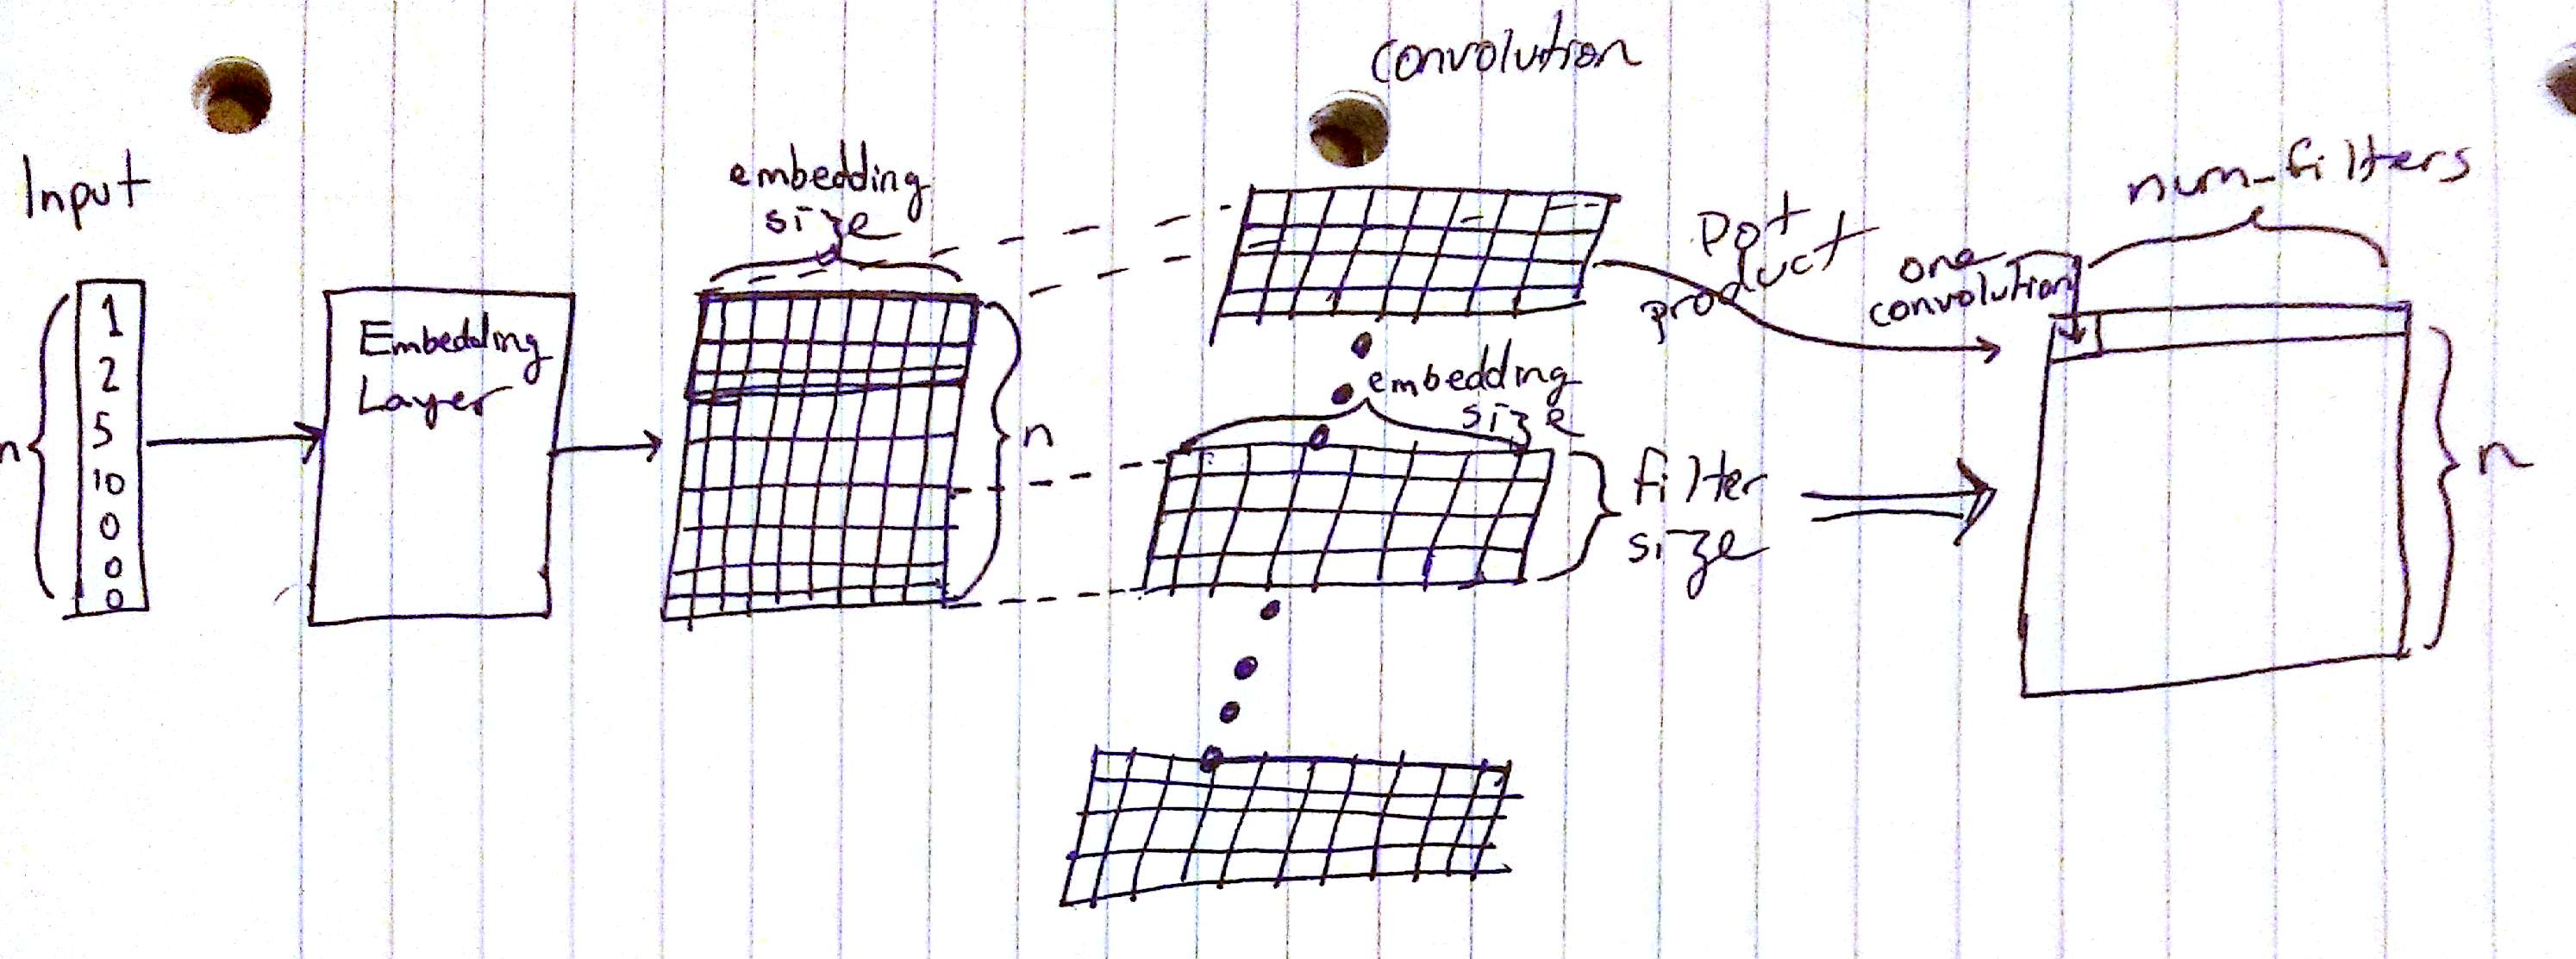
\includegraphics[height=2in, width=4in]{Images/net_conv_figure.jpg}
\caption{We apply convolution operations, sliding filters vertically to capture word context.}
\end{figure}

\subsection{ACM Abstracts: Communities of Practice Data}
We use a convolutional neural network to classify abstract text corresponding to three communities of practice: CyberSecurity,
Smart Cities, and Undergraduate Research.


\begin{figure}[H]
\centering
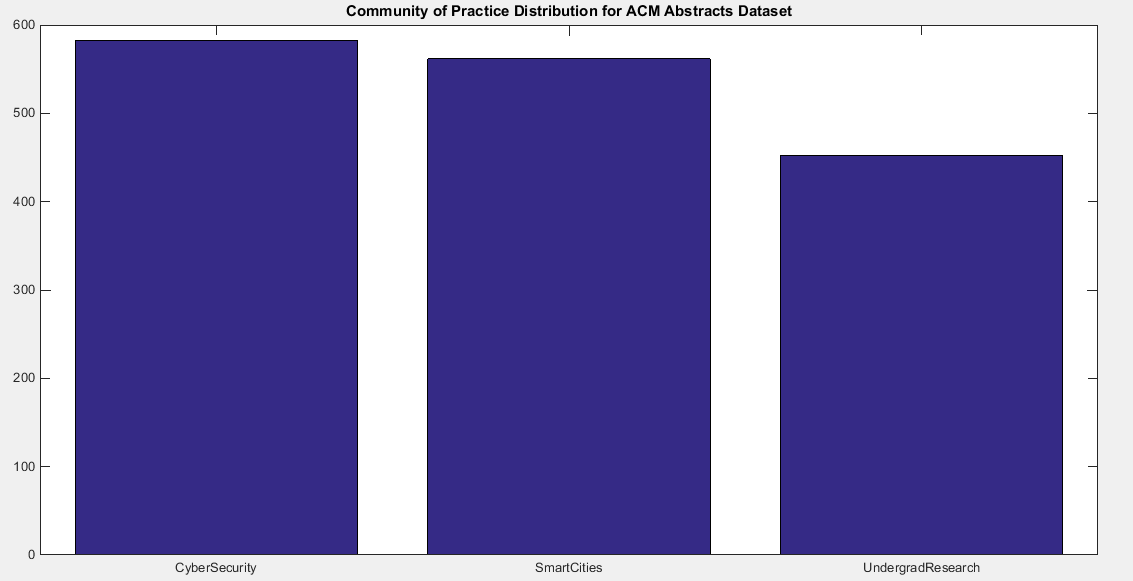
\includegraphics[height=2in, width=4in]{Images/ACM_CoP_distribution.png}
\caption{Class distribution of ACM abstract dataset.}
\end{figure}


\begin{tabular}[pos]{l c c}
  Model & Accuracy & F-Measure\\
  TF+SVM & 0.868475991649 & 0.881613394858\\
  Baseline ConvNet & 87682672246264015 & 0.87154599781573938\\
  Embedding, Conv, LSTM & PENDING & PENDING\\
\end{tabular}

\subsection{NSF Research Award Abstracts Data}
In the following section we provide a performance analysis using the NSF research award abtracts dataset.

\begin{figure}[H]
\centering
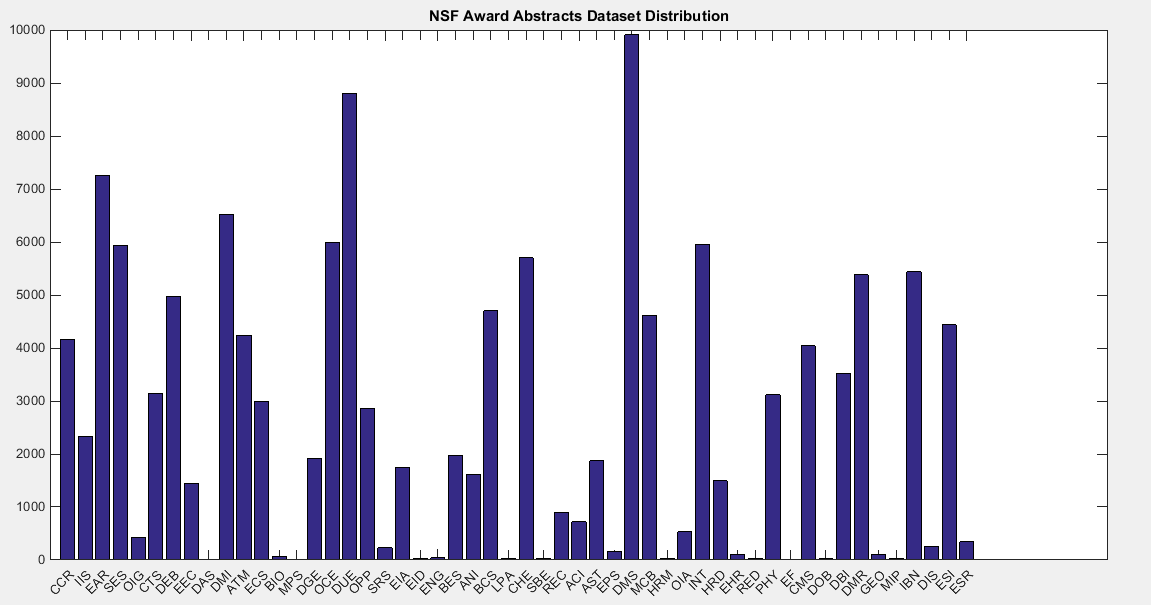
\includegraphics[height=2in, width=4in]{Images/NSF_Awards_distribution.png}
\caption{Class distribution of NSF abstract dataset.}
\end{figure}

\begin{tabular}[pos]{l c c}
  Model & Accuracy & F-Measure\\
  TF+SVM &  0.743238287338 &  0.530289948052\\
  Baseline ConvNet (10000, 500) & 0.8112 & 0.8193\\
  LSTM Convnet (10000, 500)& .8216 & .8277\\
\end{tabular}

\begin{figure}[H]
\centering
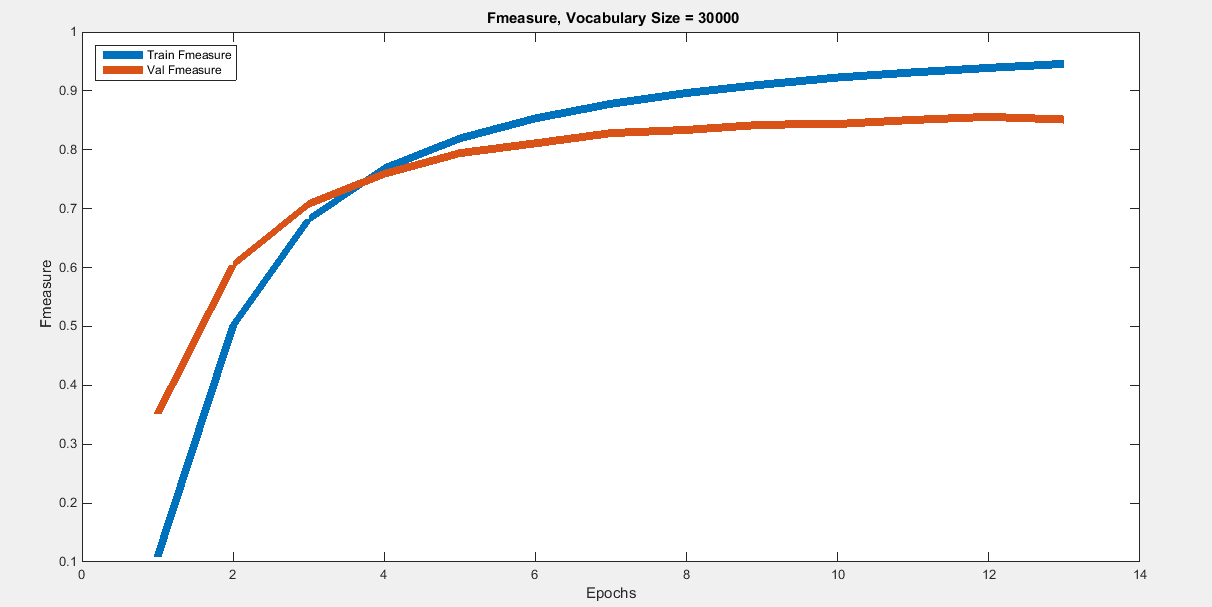
\includegraphics[height=2in, width=4in]{Images/fmeasure_nsf_30000_1000.png}
\caption{Performance plot on validation set. Vocabulary size is 30000 words, sequence length is 1000.}
\end{figure}


\begin{figure}[H]
\centering
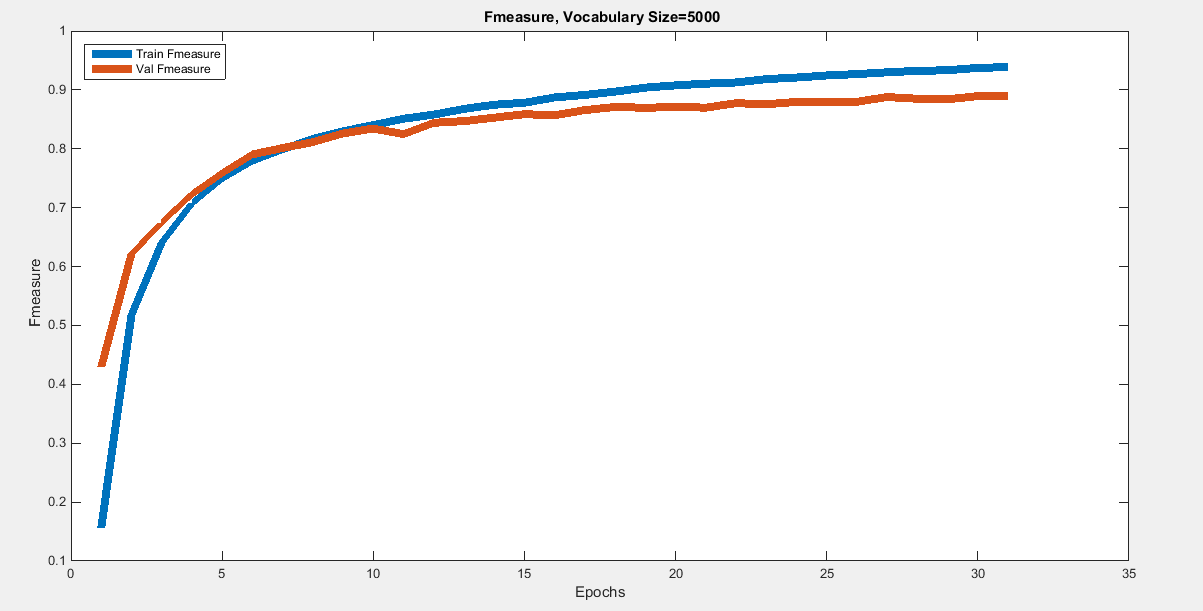
\includegraphics[height=2in, width=4in]{Images/fmeasure_nsf_5000_500.png}
\caption{Performance plot on validation set. Vocabulary size is 30000 words, sequence length is 1000.}
\end{figure}

\begin{figure}[H]
\centering
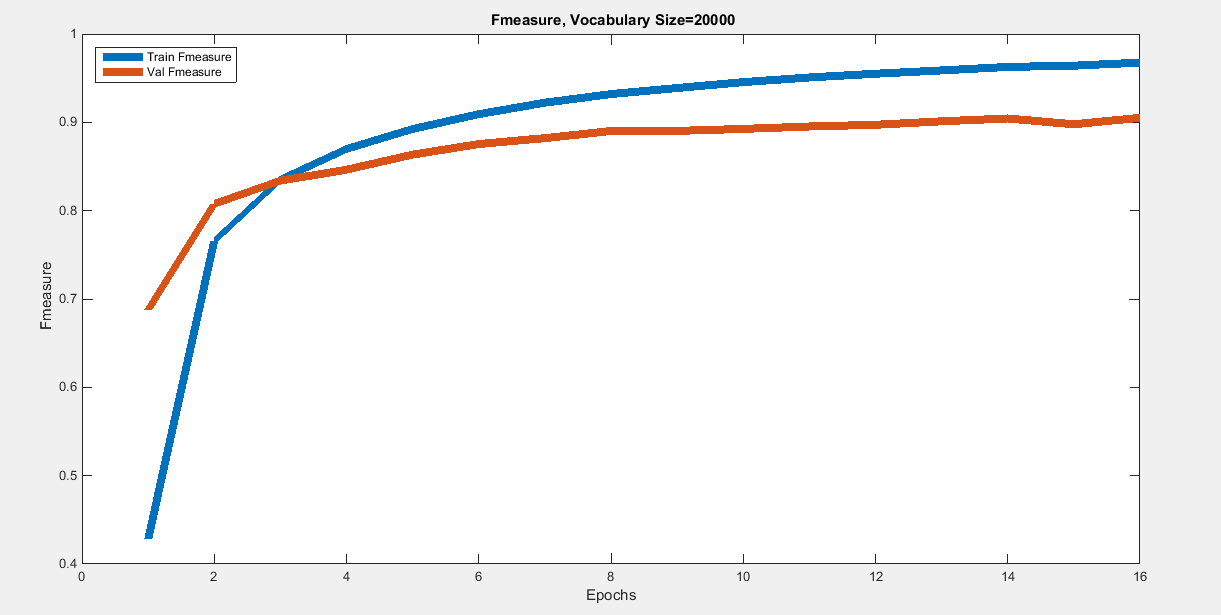
\includegraphics[height=2in, width=4in]{Images/fmeasure_nsf_20000_250.png}
\caption{Performance plot on validation set. Vocabulary size is 20000 words, sequence length is 250.}
\end{figure}

\begin{figure}[H]
\centering
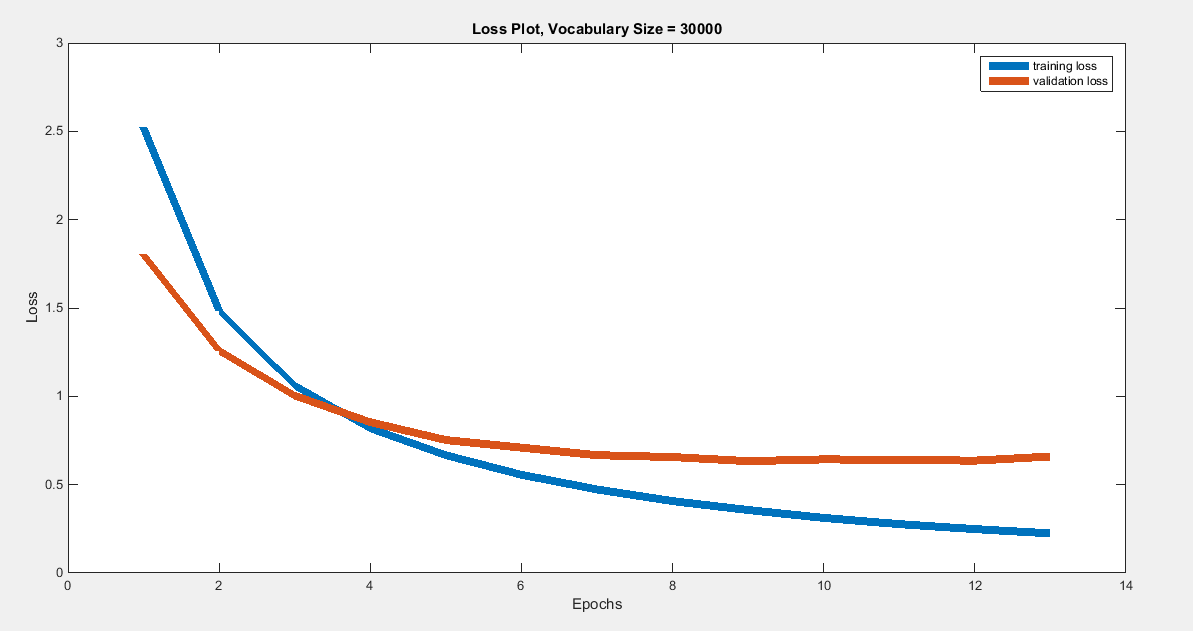
\includegraphics[height=2in, width=4in]{Images/loss_nsf_30000_1000.png}
\caption{Loss plot on validation set. Vocabulary size is 30000 words, sequence length is 1000.}
\end{figure}

\begin{figure}[H]
\centering
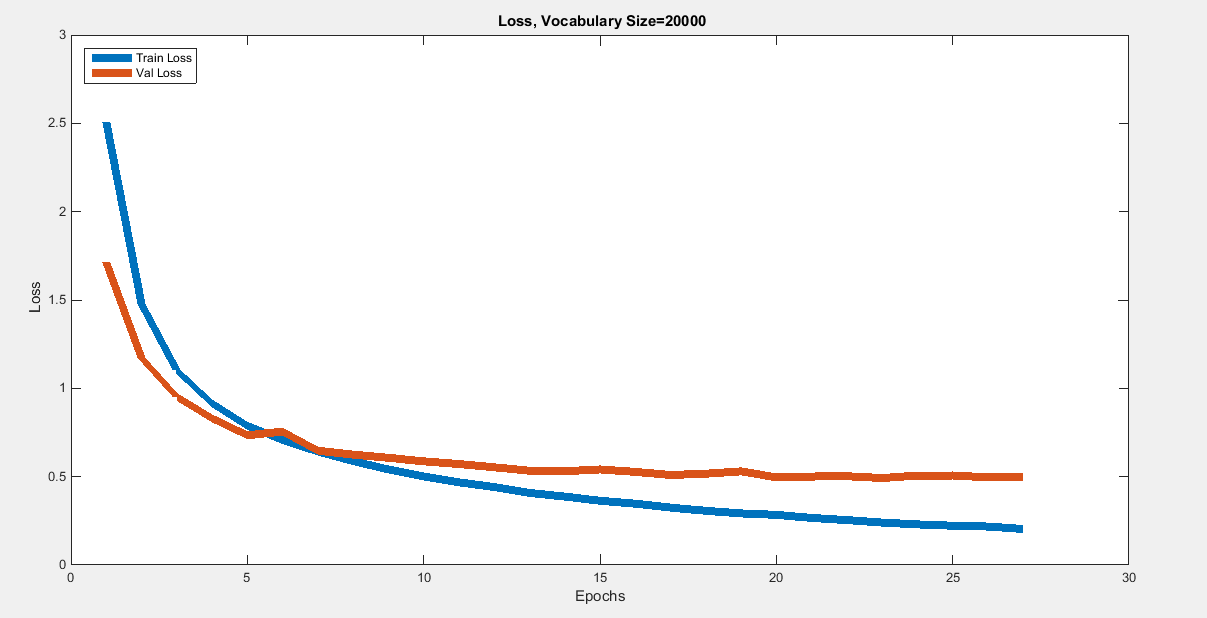
\includegraphics[height=2in, width=4in]{Images/loss_nsf_10000_500.png}
\caption{Loss plot on validation set. Vocabulary size is 10000 words, sequence length is 500.}
\end{figure}


\begin{figure}[H]
\centering
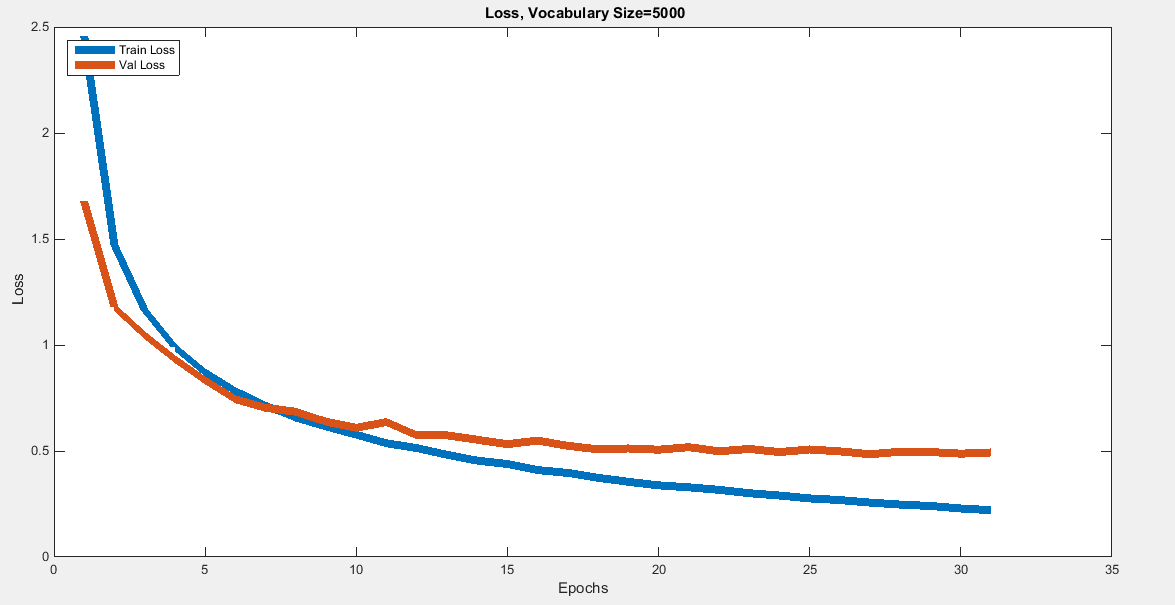
\includegraphics[height=2in, width=4in]{Images/loss_nsf_5000_500.png}
\caption{Loss plot on validation set. Vocabulary size is 5000 words, sequence length is 500.}
\end{figure}

\begin{figure}[H]
\centering
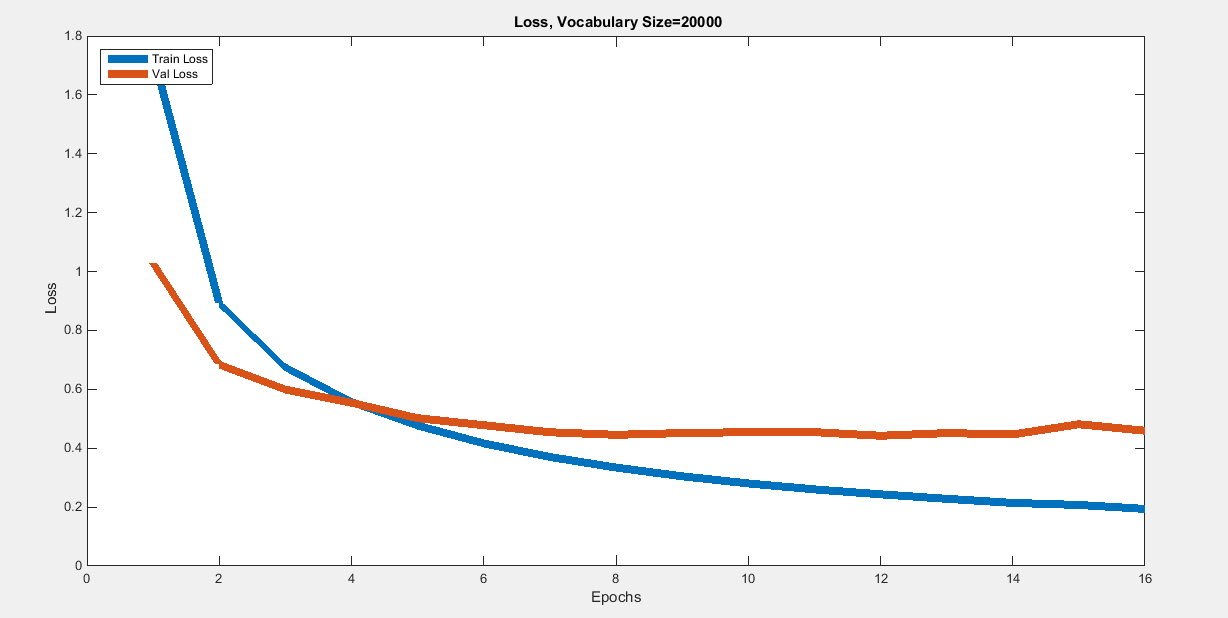
\includegraphics[height=2in, width=4in]{Images/loss_nsf_20000_250.png}
\caption{Loss plot. Vocabulary size is 20000 words, sequence length is 250.}
\end{figure}

\subsection{Arxiv Abstracts Data}
We scrape a publication abstract dataset from Arxiv.com. It is comprised of 42 computer science topics, with up to 5000 abstracts from
each topic.

\begin{figure}[H]
\centering
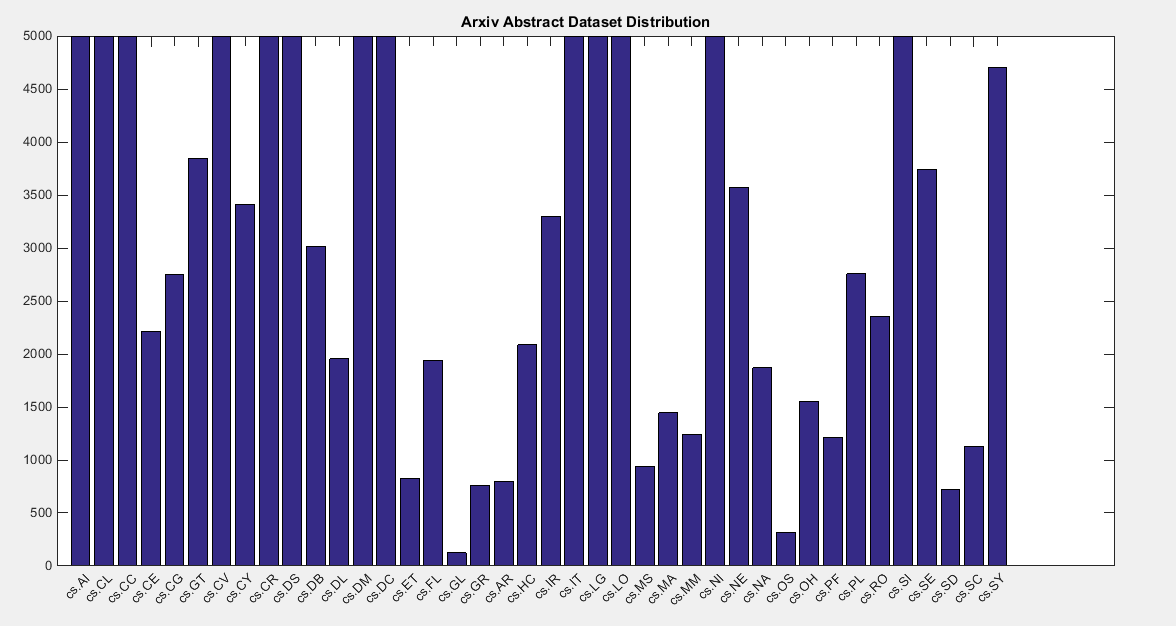
\includegraphics[height=2in, width=4in]{Images/arxiv_distribution.png}
\caption{Class distribution in the Arxiv abstract dataset. There are 40 computer science related topics, with up to 5000 publications in a topic.}
\end{figure}

\begin{figure}[H]
\centering
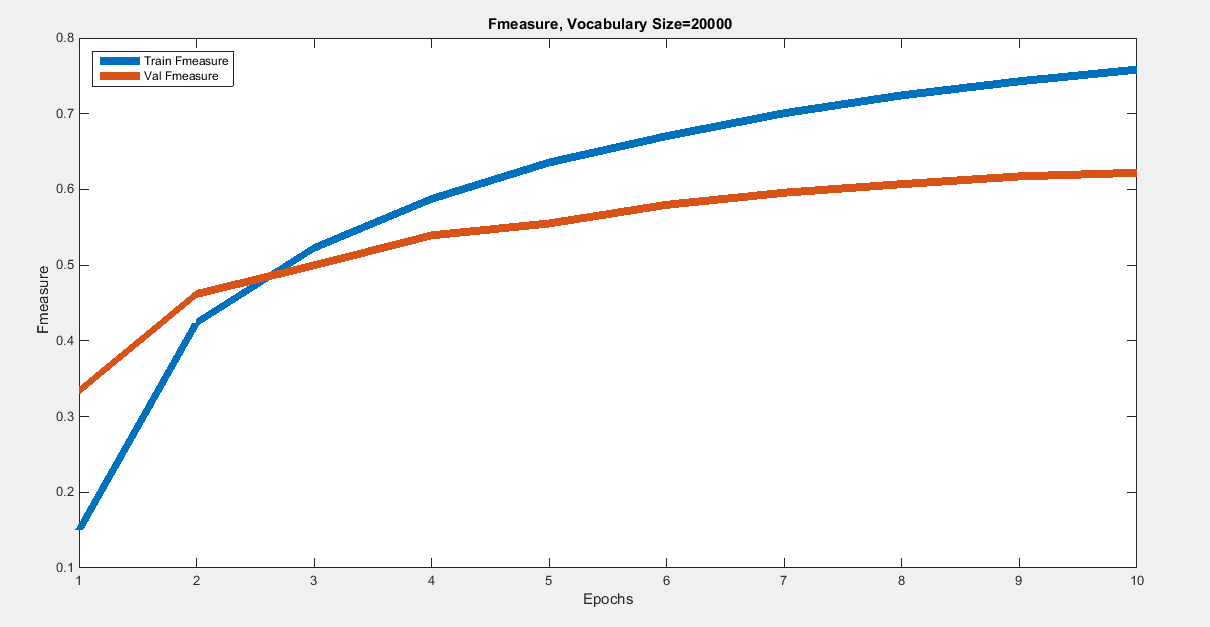
\includegraphics[height=2in, width=4in]{Images/fmeasure_arxiv_20000_150.png}
\caption{Performance plot on Arxiv data. Vocabulary size is 20000 words, sequence length is 150.}
\end{figure}

\begin{figure}[H]
\centering
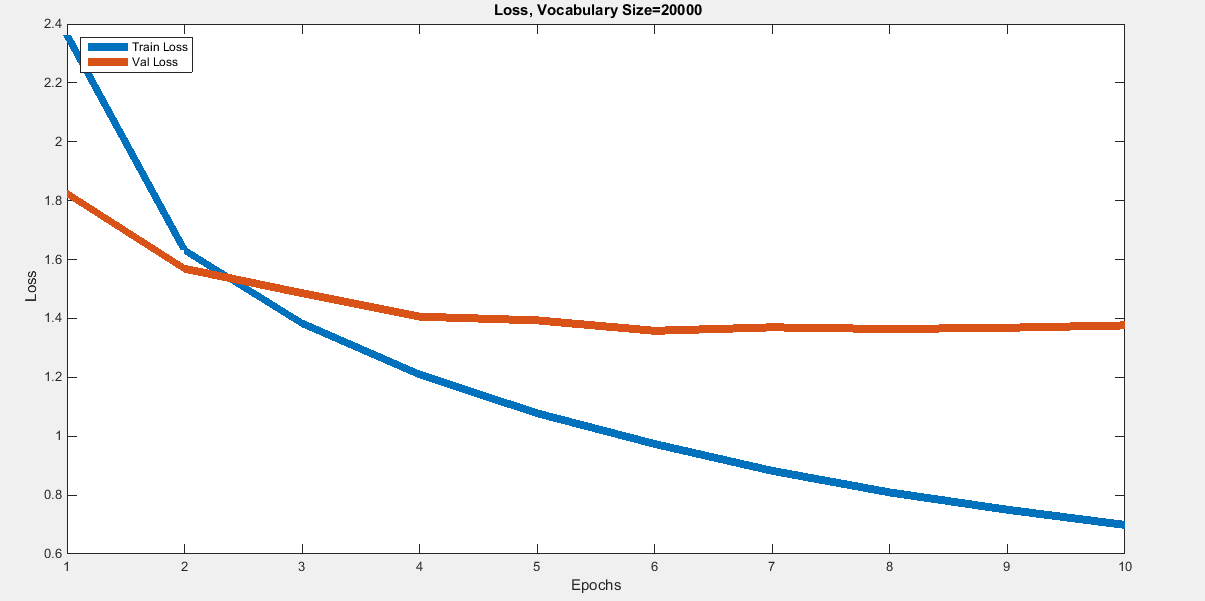
\includegraphics[height=2in, width=4in]{Images/loss_arxiv_20000_150.png}
\caption{Loss plot on Arxiv data. Vocabulary size is 20000 words, sequence length is 150.}
\end{figure}

PENDING
Add class weights for training with clas imbalance

\section{CSM Features and Layer}

PENDING

Algorithm 1 describes a keyword noun phrase extraction method for a set of noun phrases corresponding to a sentence in a document. We repeat this
algorithm and extract a noun phrase for all sentences in a document. Instead using a sequence of word indexes over the entire text, we use a sequence
of indexes over all extracted noun phrases. We use these sequences as input to the neural network.

PENDING WORK
We initialize the filters in the first feature maps to windows of the embeddings.

\section{Data Augmentation}
Data augmentation is a common practice in deep learning when a training set is not of large size. It involves a series of small random
transformation to each data sample so the network recieves new, unseen instances when training. The transformations must be somewhat substle
as to retain the overall structure of the original data. We experiment with augmenting our dataset by shuffling the order of words in windows of size 2 to
5, window size chosen at random at the beginning of a training epoch.

\begin{figure}[H]
\centering
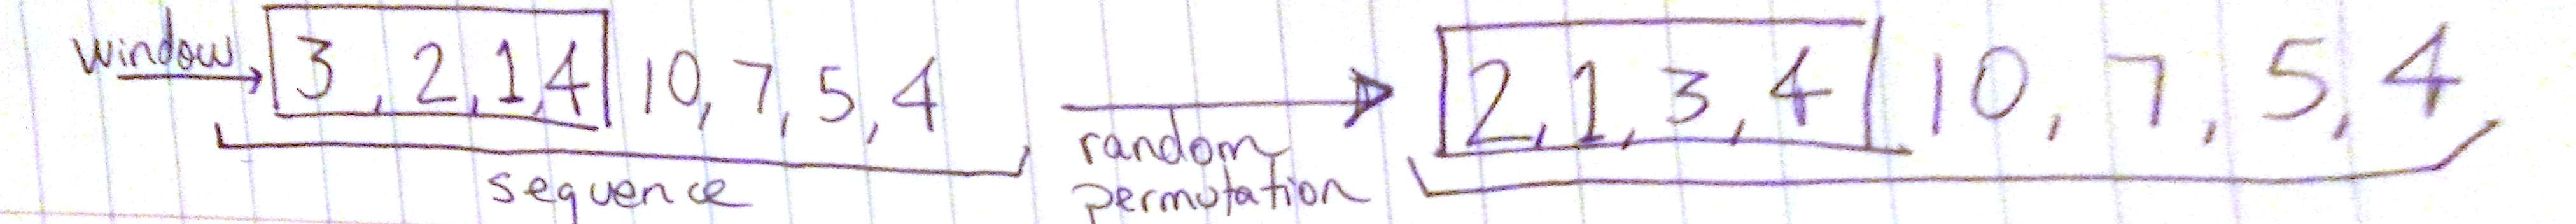
\includegraphics[height=.5in, width=4in]{Images/data_augmentation.jpg}
\caption{Example of data augmentation. We apply random permutations of the word indexes on windows of size 2 to 5, randomly chosen at the beginning of
each training epoch. Here a window of 4 is applied.}
\end{figure}


\section{Conclusion}
We presented an embedding based feature representation of documents for classification tasks using a subset of noun phrases selected using cosine
similarity minimization. We also provide an analysis of embedding based features with convolutional neural network on multiple abstract datasets.
We also develop and analyse a convolutional layer based on cosine similarity minimization and discuss the effects of data augmentation on text data.

\end{document}
